
\documentclass[12pt]{article}
\usepackage{graphicx}
\usepackage{amsmath}
\usepackage{mathtools}
\usepackage{gensymb}
\usepackage{tabularx}
\usepackage{array}
\usepackage[latin1]{inputenc}
\usepackage{fullpage}
\usepackage{color}
\usepackage{array}
\usepackage{longtable}
\usepackage{calc}
\usepackage{multirow}
\usepackage{hhline}
\usepackage{ifthen}
\usepackage{lscape}
\usepackage{float}
\usepackage{amssymb}

\newcommand{\mydet}[1]{\ensuremath{\begin{vmatrix}#1\end{vmatrix}}}
\providecommand{\brak}[1]{\ensuremath{\left(#1\right)}}
\providecommand{\norm}[1]{\left\lVert#1\right\rVert}
\providecommand{\abs}[1]{\left\vert#1\right\vert}
\newcommand{\solution}{\noindent \textbf{Solution: }}
\newcommand{\myvec}[1]{\ensuremath{\begin{pmatrix}#1\end{pmatrix}}}
\let\vec\mathbf

\def\inputGnumericTable{}

\begin{document}
\begin{center}
\textbf\large{OPTIMIZATION}

\end{center}
\section*{Excercise 6.6}

Q4. Find the equation of normal to the curve $x^2=4y$ which passes through the point (4,-2)

\solution
The given equation of the curve can be written as  
\begin{align}
	\label{eq:parabolaEq2}
	g\brak{\vec{x}} = \vec{x}^\top\vec{V}\vec{x} + 2\vec{u}^\top\vec{x} + f = 0 
\end{align}
where
\begin{align}
	\label{eq:eqV}
	\vec{V} &= \myvec{ 1 & 0 \\ 0 & 0} \\
	\label{eq:eqU}
	\vec{u} &= \myvec{0 \\ -2} \\
	\label{eq:eqF}
	f &= 0 
\end{align}
We are given that 
\begin{align}
	\vec{h} &= \myvec{4 \\ -2}
\end{align}
This can be formulated as optimization problem as follows:
\begin{align}
	\label{eq:Eq3}
	&  \min_{\vec{x}} \quad \text{f}\brak{\vec{x}} = \norm{\vec{x}-\vec{h}}^2\\
	\label{eq:Eq4}
	& \text{s.t.}\quad g\brak{\vec{x}} = \vec{x}^\top\vec{V}\vec{x} + 2\vec{u}^\top\vec{x} + f = 0  
\end{align}
First we check whether \eqref{eq:Eq4} is convex or not. Assume $\vec{x}_1 \text{ and } \vec{x}_2$ that satisfy $g\brak{\vec{x}}=0$. Then,
\begin{align}
	\label{eq:eq5}
	g\brak{\vec{x}_1} = \vec{x}_1^\top\vec{V}\vec{x}_1+2\vec{u}^\top\vec{x}_1+f=0\\
	\label{eq:eq6}
	g\brak{\vec{x}_2} = \vec{x}_2^\top\vec{V}\vec{x}_2+2\vec{u}^\top\vec{x}_2+f=0\\
\end{align}
Then, for any $0\le\lambda\le1$, we substitute
\begin{align}
	\vec{x}_\lambda = \lambda\vec{x}_1+\brak{1-\lambda}\vec{x}_2
\end{align}
into \eqref{eq:Eq4}, we get
\begin{align}
        \label{eq:Eq5}
	g\brak{\vec{x}_\lambda} = \brak{\lambda\vec{x}_1+\brak{1-\lambda}\vec{x}_2}^\top\vec{V} \brak{\lambda\vec{x}_1+\brak{1-\lambda}\vec{x}_2} + 2\vec{u}^\top\brak{\lambda\vec{x}_1+\brak{1-\lambda}\vec{x}_2} +f \\
	\implies 
	\brak{\lambda\vec{x}_1^\top+\brak{1-\lambda}\vec{x}_2^\top}\brak{\lambda\vec{V}\vec{x}_1+\brak{1-\lambda}\vec{V}\vec{x}_2}+2\lambda\vec{u}^\top\vec{x}_1+2\brak{1-\lambda}\vec{u}^\top\vec{x}_2 +f
\end{align}
\begin{multline}
	\label{eq:eq7}
	\implies 
	\lambda^2\vec{x}_1^\top\vec{V}\vec{x}_1+\lambda\vec{x}_2^\top\vec{V}\vec{x}_1-\lambda^2\vec{x}_2^\top\vec{V}\vec{x}_1+ \lambda\vec{x}_1^\top\vec{V}\vec{x}_2+\vec{x}_2^\top\vec{V}\vec{x}_2 -\lambda\vec{x}_2^\top\vec{V}\vec{x}_2-\lambda^2\vec{x}_1^\top\vec{V}\vec{x}_2\\
	-\lambda\vec{x}_2^\top\vec{V}\vec{x}_2+\lambda^2\vec{x}_2^\top\vec{V}\vec{x}_2+ 2\lambda\vec{u}^\top\vec{x}_1+2\vec{u}^\top\vec{x}_2-2\lambda\vec{u}^\top\vec{x_2} +f
\end{multline}
Multiplying \eqref{eq:eq5} by $\lambda$ and \eqref{eq:eq6} by $\brak{1-\lambda}$ and adding
\begin{multline}
	\label{eq:eqf}
	\lambda g\brak{\vec{x}_1}+ \brak{1-\lambda}g\brak{\vec{x}_2} = \lambda\vec{x}_1^\top\vec{V}\vec{x}_1 + 2\lambda\vec{u}^\top\vec{x}_1 + \lambda f + \vec{x}_2^\top\vec{V}\vec{x}_2+2\vec{u}^\top\vec{x}_2+f\\ 
	-\lambda\vec{x}_2^\top\vec{V}\vec{x}_2+2\lambda\vec{u}^\top\vec{x}_2-\lambda f = 0 \\
	\implies f = 
	-\lambda\vec{x}_1^\top\vec{V}\vec{x}_1 - 2\lambda\vec{u}^\top\vec{x}_1 -\vec{x}_2^\top\vec{V}\vec{x_2}-2\vec{u}^\top\vec{x}_2\\ 
	+\lambda\vec{x}_2^\top\vec{V}\vec{x}_2-2\lambda\vec{u}^\top\vec{x}_2
\end{multline}
Substituting the value of $f$ from \eqref{eq:eqf} in \eqref{eq:Eq5} and simplifying
\begin{align}
	\label{eq:Eq6}
	\eqref{eq:Eq5} \implies \brak{\vec{x}_1-\vec{x}_2}^\top\vec{V}\brak{\vec{x}_1-\vec{x}_2} 
\end{align}
Since $\vec{V}$ is a semi-definite matrix,the value of \eqref{eq:Eq6} will be $\ge 0$ contracdicting the equality in \eqref{eq:Eq4}. 
Hence, the optimization problem is nonconvex. However, by relaxing the constraint in \eqref{eq:Eq4} as
\begin{align}
	\label{eq:Eq7}
	& g\brak{\vec{x}} = \vec{x}^\top\vec{V}\vec{x} + 2\vec{u}^\top\vec{x} + f \le 0  
\end{align}
the optimization problem can be made convex. Applying convexity property to \eqref{eq:Eq7} and simplifying, \eqref{eq:Eq6} yields to
\begin{align}
	\label{eq:Eq8}
	\brak{\vec{x}_1-\vec{x}_2}^\top\vec{V}\brak{\vec{x}_1-\vec{x}_2} \ge 0 
\end{align}
Hence the revised constraint makes it a convex optimization problem. Solving the problem using \textit{cvxpy} we get the following point on the curve
\begin{align}
	\vec{X} = \myvec{1.695\\0.718}
\end{align}
See figure \ref{fig:Fig1}
\begin{figure}[!h]
	\begin{center} 
	    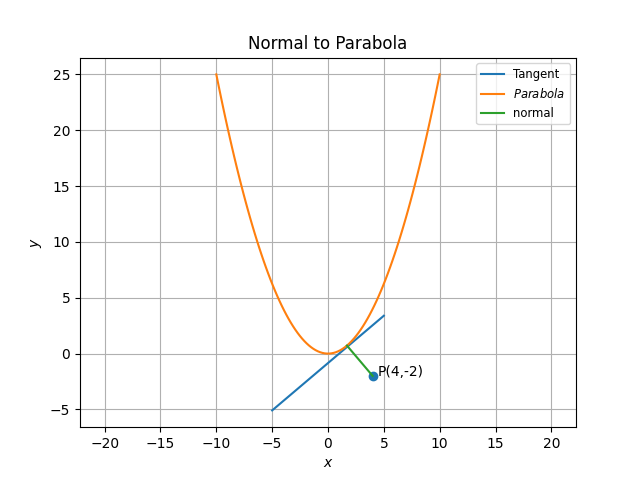
\includegraphics[width=\columnwidth]{figs/12_6_6_4}
	\end{center}
\caption{}
\label{fig:Fig1}
\end{figure}


\end{document}










































